% CMSC 197-1. Machine Learning. Mini Project Proposal
% Submitted by: Alyssa Alexandra Lee, Aren Deza, Victor Sumbong

% This is the documentclass used in ma'am's sample. 
% It makes the title and authors appear at the top of each page, so that it's easier to read when printed.
\documentclass[runningheads]{llncs}

% Formatting packages
\usepackage{indentfirst, float, graphicx, hyperref}
% Reference packages
\usepackage[square, sort, comma, numbers]{natbib}

\graphicspath{{figures/}}
\newcommand{\nocontentsline}[3]{}
\newcommand{\notoc}[2]{\bgroup\let\addcontentsline=\nocontentsline#1{#2}\egroup}

\title{\textbf{\LARGE A Comparative Study on Lung Cancer Prediction using Naïve Bayes and Logistic Regression}}

\author{Alyssa Alexandra Lee\inst{1} \texttt{aslee2@up.edu.ph} \and
\\ Aren Deza\inst{1} \texttt{apdeza1@up.edu.ph} \and
\\ Joseph Victor Sumbong\inst{1} \texttt{jssumbong@up.edu.ph} \and
\\ Ara Abigail Ambita\inst{1}}

\usepackage{fancyhdr}
\pagestyle{fancy}
\renewcommand{\headrulewidth}{0pt}
\lhead[\small \thepage \ \ A. Lee et al.]{}
\rhead[]{\small Lung Cancer Prediction using Naïve Bayes and Logistic Regression \ \ \thepage}
\cfoot{}  
\lfoot[\small \href{https://github.com/Aren-Deza/GroupL-MP197}{Github Link}]{}
\rfoot[]{\small \href{https://www.kaggle.com/datasets/thedevastator/cancer-patients-and-air-pollution-a-new-link}{Dataset Used}}

\authorrunning{A. Lee et al.}
\titlerunning{Lung Cancer Prediction using Naïve Bayes and Logistic Regression}
\institute{University of The Philippines Visayas, Miag-ao, Iloilo City}

\begin{document}
\maketitle

\pagenumbering{roman}
\pagenumbering{arabic}

\begin{abstract}
Lung cancer is the 2nd leading type of cancer in the Philippines, and has the highest mortality rate among all cancer types. As it is important to diagnose and treat lung cancer cases as early as possible, the researchers sought to  implement and compare Machine learning models that can identify an individual’s likelihood of developing lung cancer and determine the top 3 factors for people with high, medium, and low likelihood of contracting lung cancer. The study used a modified dataset of information on patients with lung cancer. After successfully implementing and comparing both models, it was found that Logistic Regression provided a more effective model for predicting risk of developing lung cancer, with 98.4\% accuracy and 98\% macro average for precision, recall and f1-score. The researchers also identified the top three predictors for each level of risk, with fatigue, passive smoking, and exposure to air pollution being strongly correlated with high risk; fatigue, passive smoking, and coughing of blood being correlated with medium risk; and fatigue, clubbing of fingernails, and wheezing having a strong negative correlation with low risk.


\keywords{Machine learning \and Lung cancer \and Logistic Regression \and Naive Bayes.}
\end{abstract}

\section{Introduction}

\subsection{Background of the Study}
Lung cancer is a disease characterized by a malignant growth or tumor formed from the uncontrollable division of abnormal cells, specifically within the lungs \cite{cancerResearchUK2019}. It is known to be the most common type of cancer and is also the main cause of cancer death globally. The chance to get and develop this disease increases with a myriad of factors such as tobacco smoking, exposure to chemicals in the workplace, long-term exposure to air pollution, exposure to radon gas, having a family history of lung cancer, etc.

In the Philippines, it is common to encounter a person smoking as you walk down the street. According to MacroTrends \cite{macrotrends2022}, the prevalence of Filipino smokers aged 15 and above on a daily or non-daily basis is 22.90\% in the year 2020. The population density in the Philippines is also greatest in the National Capital Region with 21,765 persons per square kilometer \cite{philippinestatisticsauthority2021}. This region also accounts for 13,484,462 persons of the 109,033,245 or 12.37\% total population of the country. In NCR, the most densely populated city was Manila with 73,920 persons per square kilometer. According to IQAir \cite{IQAir2022}, in 2019, Manila had an average of 18.2 µg/m³ of PM2.5 or particulate matter under 2.5 micrometers which poses health concerns. This recording placed them under the “Moderate” category of the World Health Organization (WHO). However, with the lockdown being lifted and traffic becoming more of a problem, the air quality is forecasted to worsen. In a press release by the  Department of Health in 2022 \cite{doh2021}, Lung cancer is the 2nd leading type of cancer in the country and is the leading cause of mortality in all cancer types. 

If it is identified and diagnosed in its earliest stages, lung cancer can fortunately be treated. However, a patient suffering from lung cancer can be asymptomatic while the disease is in its earlier stages of progression, which can make it difficult to detect. For this reason, having the ability to quickly and reliably predict whether a patient may have or is at risk of contracting lung cancer can be invaluable in reducing their chances of dying from the disease. 
Therefore, the researchers aim to employ machine learning technologies to identify significant factors among lung cancer patients and construct a model that can be used to predict and evaluate an individual's risk of contracting the disease while choosing the best machine learning algorithm that the researchers have learned. 

There have been studies such as “A Study On Prediction Of Lung Cancer Using Machine Learning Algorithms” by Ahmad et al. \cite{gupta2022} which compared 3 machine learning algorithms in their ability to predict lung cancer, however, their dataset was biomedical images and they had an image processing step. Other similar studies also used a collection of labeled images for their dataset. A similar study that did not utilize an image dataset is “A Comparative Study of Lung Cancer Detection using Machine Learning Algorithms” by Radhika et al. \cite{radhika2019} It utilized Support Vector Machine (SVM), Logistic Regression, Naïve Bayes, and Decision Tree machine learning algorithms as well as a different dataset than the researchers will use. This paper differs from the aforementioned study due to its different dataset as well as the machine learning algorithms that will be utilized and compared.

\subsection{Statement of the Problem}
The researchers will implement and compare Machine learning models that can identify an individual’s likelihood of developing lung cancer. Specifically, the researchers will:
\begin{enumerate}
	\item train a Logistic Regression model to predict likelihood of lung cancer;
	\item train a Naive Bayes model to predict likelihood of lung cancer;
	\item compare Naive Bayes and Logistic Regression’s evaluation scores;
	\item determine the top 3 factors for people with high likelihood of contracting lung cancer; 
	\item determine the top 3 factors for people with medium likelihood of contracting lung cancer; and
	\item determine the top 3 factors for people with low likelihood of contracting lung cancer.
\end{enumerate}

\subsection{Hypothesis}
The researchers will not be able to implement a Machine learning model that can identify an individual’s likelihood of developing lung cancer.

\subsection{Scope and Delimitation}
The scope of this paper is to determine only lung cancer likelihood using the dataset of the user, “The Devastator”, from the website, Kaggle. It will also only implement and compare Naive Bayes and Logistic Regression as its Machine Learning models. The researchers will make use of the following tools: (1) Jupyter Notebook, (2) Google Docs, (3) Github, and (4) TeXworks. The LaTeX packages used are the following: (1) indentfirst, (2) float, (3) graphicx, (4) hyperref, (5) fancyhdr, and (6) natbib. The Python packages that will be employed are: (1) Pandas, (2) NumPy, (3) scikit-learn, and (4) Matplotlib which will be used in implementing the models.

The paper will not use any other dataset aside from the one mentioned above. It will also not predict whether a patient has lung cancer or not, but rather only the patient’s likelihood of developing lung cancer. Additionally, it will not predict the likelihood of other types of cancer. It will only use the following features: (1) age; (2) gender; (3) level of air pollution exposure; (4) level of alcohol use; (5) level of dust allergy; (6) level of occupational hazards; (7) level of genetic risk; (8) level of chronic lung disease; (9) level of balanced diet; (10) level of obesity; (11) level of smoking; (12) level of passive smoker; (13) level of chest pain; (14) level of coughing of blood; (15) level of fatigue; (16) level of weight loss; (17) level of shortness of breath; (18) level of wheezing; (19) level of swallowing difficulty; (20) and level of clubbing of finger nails.

\section{Methodology}

\subsection{Dataset}
The dataset contains information on patients with lung cancer. This includes background information such as their age, gender, exposure to air pollution, alcohol use, occupational hazards, genetic risk, balanced diet, obesity, history of smoking or passive smoking, and presence of dust allergies and chronic lung disease. It also provides data of their lung cancer symptoms based on severity, which includes chest pain, coughing of blood, fatigue, weight loss, shortness of breath, wheezing, difficulty swallowing, clubbing of finger nails, snoring, and the level of lung cancer. This dataset was retrieved from the website, Kaggle.

To use this dataset for the purpose of this study, the researchers excluded the columns of \textit{Patient Id, Frequent Cold, Snoring,} and \textit{Dry Cough}. The remaining columns excluding Level are designated as the features that are of interest, while the Level column values are used as the true label. The values of the features were then standardized. The manipulated dataset was then split with a 1:3 ratio, resulting in 75\% of the entries being the training set and 25\% being the testing set. 

\subsection{Implementation of Machine Learning Models}
The machine learning models to be used in this paper are Logistic Regression and Naive Bayes. The scikit-learn library was used to create these models, specifically, the Logistic Regression function for the creation of the Logistic Regression Model which is not only binary but is able to predict multiple outcomes, and the GaussianNB function for the creation of the Naive Bayes model which can also predict multiple outcomes. They were both trained using the same training set as mentioned in the Dataset portion of this paper.

\subsection{Metrics of Evaluation}
Each of the created model’s performance was measured based on their accuracy, precision, recall, f1-score, and confusion matrix for both their training and testing sets. The evaluation was done using sklearn’s accuracy\_score, classification\_report, and confusion\_matrix function, while its ConfusionMatrixDisplay function was used to show the confusion matrix.

\section{Results}

\subsection{Logistic Regression}

\begin{table}[ht]
\centering
\caption{Logistic Regression Training Set}
\begin{tabular}{|l|c|c|c|c|} \hline
 & precision & recall & f1-score & support \\ \hline
High   & 1.00 & 1.00 & 1.00 & 261 \\ \hline
Low    & 1.00 & 0.97 & 0.99 & 237 \\ \hline
Medium & 0.98 & 1.00 & 0.99 & 252 \\ \hline
& & & & \\ \hline
accuracy     & & & 0.99 & 750 \\ \hline
macro avg    & 0.99 & 0.99 & 0.99 & 750 \\ \hline
weighted avg & 0.99 & 0.99 & 0.99 & 750 \\ \hline
\end{tabular}
\label{tab:regression-training}
\end{table}

Within the training set, the Logistic Regression model possessed an accuracy of 99.2\%, with the macro average of precision, recall, and f1-score all being 99\%. 

\begin{figure}[H]           	 
\centering               	 
\caption{Confusion matrix for Linear Regression on training set}
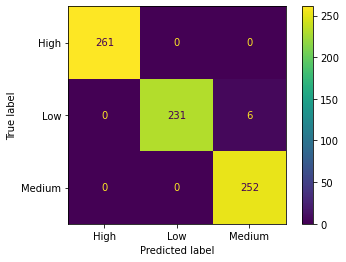
\includegraphics[scale=0.5]{regression-CM-training.png}  	 
\label{fig:regression-CM-training}
\end{figure}

The confusion matrix generated for the training set indicated that the model correctly identified all patients who had High and Low risks of lung cancer, and only mislabeling 6 patients who had a Medium risk of lung cancer as low risk.
\newpage

\begin{table}[ht]
\centering
\caption{Logistic Regression Testing Set}
\begin{tabular}{|l|c|c|c|c|} \hline
 & precision & recall & f1-score & support \\ \hline
High   & 1.00 & 1.00 & 1.00 & 104 \\ \hline
Low    & 1.00 & 0.94 & 0.97 & 66 \\ \hline
Medium & 0.95 & 1.00 & 0.98 & 80 \\ \hline
& & & & \\ \hline
accuracy     & & & 0.98 & 250 \\ \hline
macro avg    & 0.98 & 0.98 & 0.98 & 250 \\ \hline
weighted avg & 0.98 & 0.98 & 0.98 & 250 \\ \hline
\end{tabular}
\label{tab:regression-testing}
\end{table}

Meanwhile, when used on the testing set, the model had an accuracy of 98.4\%, with macro average of precision, recall, and f1-score all being 98\%. 

\begin{figure}[ht]           	 
\centering               	 
\caption{Confusion matrix for Linear Regression on testing set}
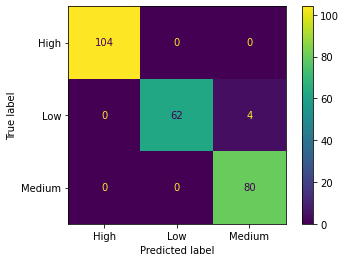
\includegraphics[scale=0.5]{regression-CM-testing.png}  	 
\label{fig:regression-CM-testing}
\end{figure}

Its generated confusion matrix displays similar results to the training set’s confusion matrix, where the model correctly identified patients with both High and Low risks of lung cancer, and only mislabeled 4 patients with Medium risk of lung cancer as low risk.

Based on the results obtained from using the model in the training and testing datasets, it can be asserted that the model is highly accurate in its predictions, and can be reliably used to identify how likely it is for a given patient to contract lung cancer.
\newpage

\subsection{Naive Bayes}

\begin{table}[ht]
\centering
\caption{Naive Bayes Training Set} \vspace{0.25em}
\begin{tabular}{|c|c|c|c|c|} \hline
 & precision & recall & f1-score & support \\ \hline
High   & 0.82 & 0.95 & 0.88 & 261 \\ \hline
Low    & 0.88 & 0.92 & 0.89 & 237 \\ \hline
Medium & 0.86 & 0.69 & 0.76 & 252 \\ \hline
& & & & \\ \hline
accuracy     & & & 0.85 & 750 \\ \hline
macro avg    & 0.85 & 0.85 & 0.85 & 750 \\ \hline
weighted avg & 0.85 & 0.85 & 0.85 & 750 \\ \hline
\end{tabular}
\label{tab:naivebayes-training}
\end{table}

In the training set, the Naive Bayes model had 84.93\% accuracy with macro average precision, recall, f1-score of 85\%. 

\begin{figure}[ht]           	 
\centering               	 
\caption{Confusion matrix for Naive Bayes on training set}
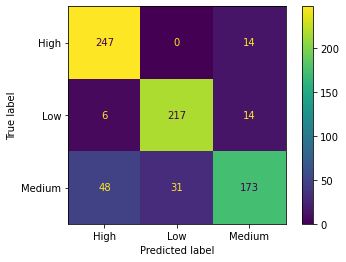
\includegraphics[scale=0.5]{naivebayes-CM-training.png}  	 
\label{fig:naivebayes-CM-training}
\end{figure}

The confusion matrix in the training set showed that the majority of the results laid on the hypotenuse which showed that it was fairly accurate in its predictions. The highest error it had in its prediction was predicting 48 Medium Risk being labeled as High Risk.
\newpage

\begin{table}[ht]
\centering
\caption{Naive Bayes Testing Set} \vspace{0.25em}
\begin{tabular}{|c|c|c|c|c|} \hline
 & precision & recall & f1-score & support \\ \hline
High   & 0.86 & 0.94 & 0.90 & 104 \\ \hline
Low    & 0.85 & 0.85 & 0.85 & 66 \\ \hline
Medium & 0.83 & 0.72 & 0.77 & 80 \\ \hline
& & & & \\ \hline
accuracy     & & & 0.85 & 250 \\ \hline
macro avg    & 0.85 & 0.84 & 0.84 & 250 \\ \hline
weighted avg & 0.85 & 0.85 & 0.85 & 250 \\ \hline
\end{tabular}
\label{tab:naivebayes-testing}
\end{table}

In the testing set, the model had an accuracy of 84.8\%, with macro average precision being 85\%, and both recall and f1-score being 84\%.

\begin{figure}[ht]           	 
\centering               	 
\caption{Confusion matrix for Naive Bayes on testing set}
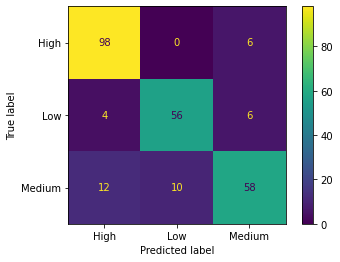
\includegraphics[scale=0.5]{naivebayes-CM-testing.png}  	 
\label{fig:naivebayes-CM-testing}
\end{figure}

The confusion matrix generated showed that it had correctly identified the majority of each class. However, the model produced some misidentifications wherein all classes whose highest mistake was 12 Medium risk were incorrectly labeled as High by the model. 

These results show that the Naive Bayes model is fairly accurate, and has the capacity to be a good model for predicting the likelihood with which a patient may contract lung cancer.

\subsection{Comparison of Models}

% Training Set

\begin{figure}[!htb]           	 
\centering               	 
\caption{Comparison Between Logistic Regression and Naive Bayes in the Training Set} \vspace{0.5em}
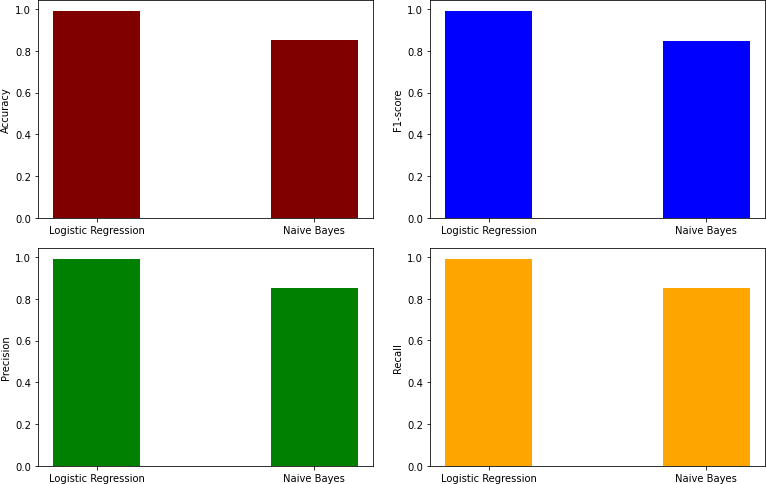
\includegraphics[scale=2]{datavis-train.png}  	 
\label{fig:datavis_train}
\end{figure}

% Testing Set

\begin{figure}[!htb]           	 
\centering          	 
\caption{Comparison Between Logistic Regression and Naive Bayes in the Testing Set} \vspace{0.5em}
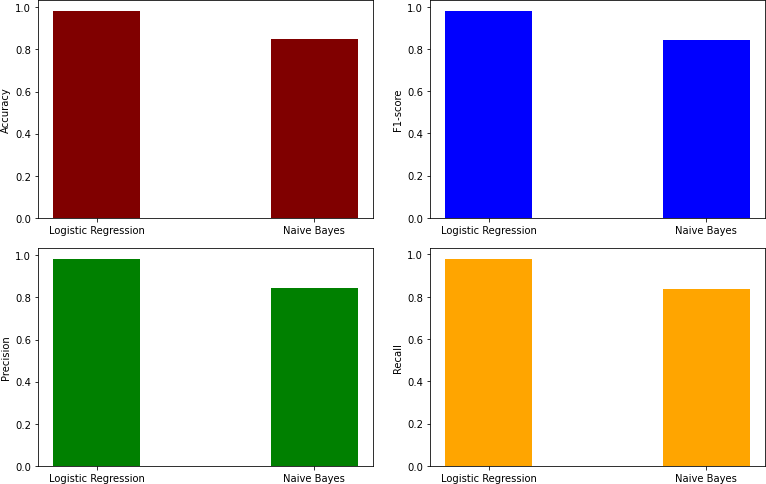
\includegraphics[scale=2]{datavis-test.png}  	 
\label{fig:datavis_test}
\end{figure}

As seen in the figures presented here, Logistic Regression gained a higher score on all metrics of evaluation on both the training and testing sets. While Naive Bayes has performed well on its own metrics, the results showed that Logistic Regression is the better algorithm for identifying an individual’s likelihood of developing lung cancer.

\subsection{Logistic Regression Feature Analysis}

\begin{figure}[!htb]           	 
\centering               	 
\caption{Correlation of Factors and High Risk}
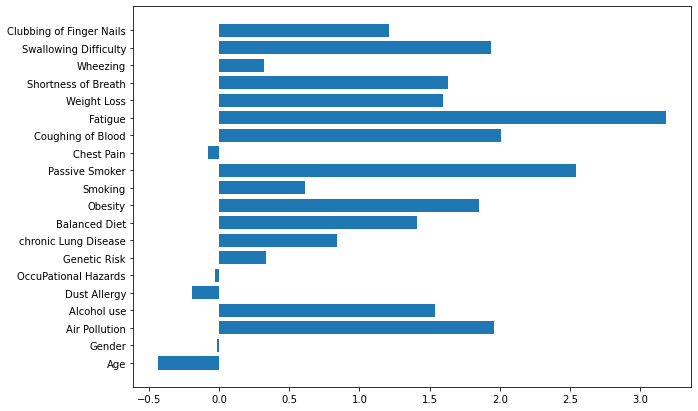
\includegraphics[scale=0.5]{fta-high.png}  	 
\label{fig:fta-high}
\end{figure}

As Logistic Regression was selected as the better model for predicting the likelihood that an individual may develop lung cancer, the weights of each feature for each class were analyzed, producing the following figures in this section.

In high risk patients (Figure \ref{fig:fta-high}), it can be observed that the top 3 factors with the strongest correlation include \textbf{Fatigue} (3.179506), \textbf{Passive Smoking} (2.541472), and \textbf{Exposure to Air Pollution} (1.960435). Each of these three features possess very strong positive correlations, with Fatigue presenting itself as the best possible predictor for a high risk of lung cancer. Findings also indicate that factors such as Chest pain, Occupational hazards, Dust allergies, and Gender possess weak negative correlations with having a high risk of lung cancer, and Age possesses a medium negative correlation with having a high risk of lung cancer.

\begin{figure}[!htb]           	 
\centering               	 
\caption{Correlation of Factors and Low Risk}
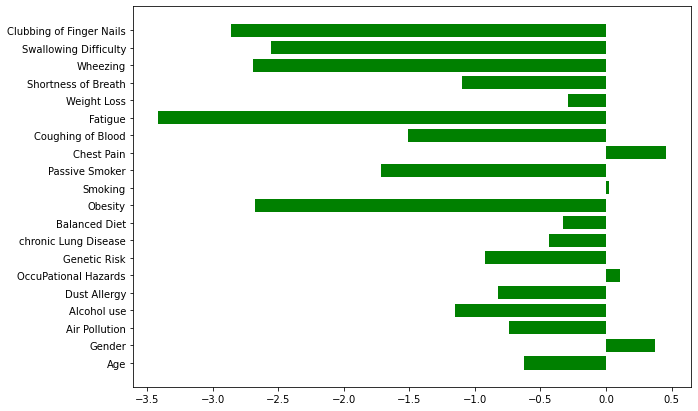
\includegraphics[scale=0.5]{fta-low.png}  	 
\label{fig:fta-low}
\end{figure}

In low risk patients (Figure \ref{fig:fta-low}), it can be observed that the top 3 factors with the highest correlation include \textbf{Fatigue} (-3.414484), \textbf{Clubbing of Finger Nails} (-2.858945), and \textbf{Wheezing} (-2.696070), each possessing strong negative correlations. The findings also show that factors such as Gender and Chest Pain possess weak positive correlations with having a low risk of lung cancer.

\begin{figure}[!htb]           	 
\centering               	 
\caption{Correlation of Factors and Medium Risk}
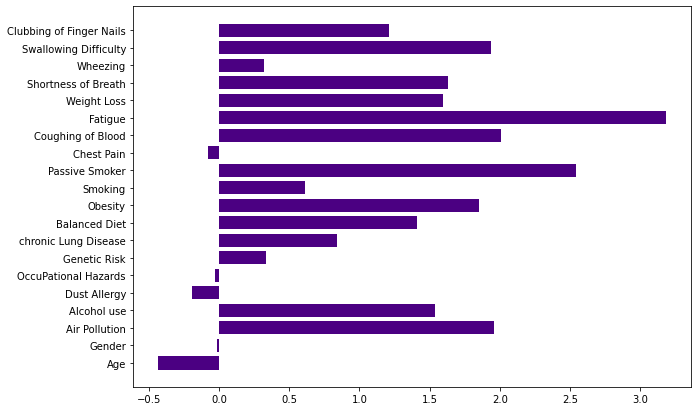
\includegraphics[scale=0.5]{fta-medium.png}  	 
\label{fig:fta-medium}
\end{figure}

In medium risk patients (Figure \ref{fig:fta-medium}), it can be observed that the top 3 factors with the highest correlation include \textbf{Fatigue} (0.234977), \textbf{Passive Smoking} (0.825177), and \textbf{Coughing of Blood} (0.498174), with each of these factors possessing strong positive correlations with a medium risk of lung cancer. It is also worth noting that factors such as Age, Dust Allergies, and Chest Pain possess weak negative correlations with a medium risk of lung cancer.
Based on what has been displayed by the findings, Fatigue has consistently displayed itself as a suitable predictor when determining a patient's risk of contracting lung cancer, displaying strong positive correlations for high and medium risk patients, and strong negative correlations for patients with low risk.

\section{Conclusion}

This study was made due to the desire of the researchers to implement and compare Machine learning models that can identify an individual’s likelihood of developing lung cancer. Specifically, they sought to: train a Logistic Regression model to predict likelihood of lung cancer; train a Naive Bayes model to predict likelihood of lung cancer; compare Naive Bayes and Logistic Regression’s evaluation scores; determine the top 3 factors for people with high likelihood of contracting lung cancer; determine the top 3 factors for people with medium likelihood of contracting lung cancer; and determine the top 3 factors for people with low likelihood of contracting lung cancer. The researchers used a modified dataset of information on patients with lung cancer for the training and testing of the machine learning models. 

At the end of the study the researchers were able to implement a Machine learning model that can identify an individual’s likelihood of developing lung cancer. Specifically, they were able to train both a Logistic Regression model and Naive Bayes model with a 98.4\% and 84.8\% accuracy score respectively in the testing set which indicates that both sets are fairly reliable in predicting an individual’s likelihood of developing lung cancer. 
	
Logistic Regression proved to be the better model in predicting the level of lung cancer in both training and testing sets. While this high accuracy of 98.4\% in the testing set may initially seem unrealistic, the precision, recall, and f1-scores also exhibited high results (98\% macro average for all mentioned measures in the testing set), showing it was capable of identifying the classes correctly which outperformed Naive Bayes in all metrics (accuracy of 84.8\% and 85\% macro average of precision, recall, and f1-score in the testing set). The imbalance is also ruled out by the fact that the dataset had a close amount of each class. These results are supported by how Logistic Regression sees much practical use as a prediction algorithm in machine learning, and is most ideal when applied to these types of problems \cite{cai2006prediction}. Therefore, it can be safely concluded that Logistic Regression models are more effective at predicting a person’s likelihood of developing lung cancer compared to Naive Bayes models.

Furthermore, the feature analysis showed that the top 3 factors that can be used to predict whether a patient has a high risk of contracting lung cancer are fatigue (3.179506), passive smoking (2.541472), and exposure to air pollution (1.960435). Meanwhile, the top 3 factors that can be used to predict whether a patient has a low risk of contracting lung cancer are fatigue (-3.414484), clubbing of finger nails (-2.858945), and wheezing (-2.696070). To predict whether a patient has a medium risk of contracting lung cancer, the top 3 factors that can be used are fatigue (0.234977), passive smoking (-0.825177), and coughing of blood (-0.498174). Based on the findings, Fatigue has consistently displayed itself as a suitable predictor when determining a patient's risk of contracting lung cancer, displaying strong positive correlations for high and medium risk patients, and strong negative correlations for patients with low risk
	
Given similar data found in the dataset, the model that was built in this study can accurately predict an individual’s likelihood of developing lung cancer. Even without the model to make predictions, the study provided pertinent information about individuals experiencing fatigue, with a history of passive smoking and exposure to air pollution.

\subsection{Recommendations}

Based on the findings and limitations of the study, the following recommendations for improvement are made:
\begin{enumerate}
\item Test other machine learning models such as SVM and Decision Trees to identify an individual’s likelihood in developing lung cancer for more comparison. 
\item Use the excluded columns of the dataset as features in training and testing the model.
\item Use other similar but larger datasets with more features but not too much in training and testing the models.
\item Delve into studying the features that showed strong positive correlation with likelihood of developing lung cancer.
\end{enumerate}

\bibliographystyle{apa}
\bibliography{Mini_Project_Bibliography}

\end{document}
